\documentclass{article}\usepackage[]{graphicx}\usepackage[]{color}
% maxwidth is the original width if it is less than linewidth
% otherwise use linewidth (to make sure the graphics do not exceed the margin)
\makeatletter
\def\maxwidth{ %
  \ifdim\Gin@nat@width>\linewidth
    \linewidth
  \else
    \Gin@nat@width
  \fi
}
\makeatother

\definecolor{fgcolor}{rgb}{0.345, 0.345, 0.345}
\newcommand{\hlnum}[1]{\textcolor[rgb]{0.686,0.059,0.569}{#1}}%
\newcommand{\hlstr}[1]{\textcolor[rgb]{0.192,0.494,0.8}{#1}}%
\newcommand{\hlcom}[1]{\textcolor[rgb]{0.678,0.584,0.686}{\textit{#1}}}%
\newcommand{\hlopt}[1]{\textcolor[rgb]{0,0,0}{#1}}%
\newcommand{\hlstd}[1]{\textcolor[rgb]{0.345,0.345,0.345}{#1}}%
\newcommand{\hlkwa}[1]{\textcolor[rgb]{0.161,0.373,0.58}{\textbf{#1}}}%
\newcommand{\hlkwb}[1]{\textcolor[rgb]{0.69,0.353,0.396}{#1}}%
\newcommand{\hlkwc}[1]{\textcolor[rgb]{0.333,0.667,0.333}{#1}}%
\newcommand{\hlkwd}[1]{\textcolor[rgb]{0.737,0.353,0.396}{\textbf{#1}}}%
\let\hlipl\hlkwb

\usepackage{framed}
\makeatletter
\newenvironment{kframe}{%
 \def\at@end@of@kframe{}%
 \ifinner\ifhmode%
  \def\at@end@of@kframe{\end{minipage}}%
  \begin{minipage}{\columnwidth}%
 \fi\fi%
 \def\FrameCommand##1{\hskip\@totalleftmargin \hskip-\fboxsep
 \colorbox{shadecolor}{##1}\hskip-\fboxsep
     % There is no \\@totalrightmargin, so:
     \hskip-\linewidth \hskip-\@totalleftmargin \hskip\columnwidth}%
 \MakeFramed {\advance\hsize-\width
   \@totalleftmargin\z@ \linewidth\hsize
   \@setminipage}}%
 {\par\unskip\endMakeFramed%
 \at@end@of@kframe}
\makeatother

\definecolor{shadecolor}{rgb}{.97, .97, .97}
\definecolor{messagecolor}{rgb}{0, 0, 0}
\definecolor{warningcolor}{rgb}{1, 0, 1}
\definecolor{errorcolor}{rgb}{1, 0, 0}
\newenvironment{knitrout}{}{} % an empty environment to be redefined in TeX

\usepackage{alltt}

\usepackage{float}

% Set the margins on the page to not be so large
\addtolength{\oddsidemargin}{-.875in}
\addtolength{\evensidemargin}{-.875in}
\addtolength{\textwidth}{1.75in}
\addtolength{\topmargin}{-.875in}
\addtolength{\textheight}{1.75in}

% Take off page numbering
\pagenumbering{gobble}
\IfFileExists{upquote.sty}{\usepackage{upquote}}{}
\begin{document}

\title{%
  Stat 5100 Handout 3.1.1 - R: Alternative Predictor Variable Types \\
  \smallskip
  \large Stat 5100: Dr. Bean
}
\date{}

\maketitle

\textbf{Example 1:} (Table 8.1)  Study looks at the effects of the charge rate and temperature on the life of a new type of power cell.  A small-scale preliminary study was conducted using 11 power cells.  Variables reported are the charge rate ($X_1$, in amperes), the ambient temperature ($X_2$, in degrees Celsius), and the life of the power cell ($Y$, in the number of discharge-charge cycles before failure).

\begin{knitrout}
\definecolor{shadecolor}{rgb}{0.969, 0.969, 0.969}\color{fgcolor}\begin{kframe}
\begin{alltt}
\hlcom{# Input data -- see Table 8.1 in text}
\hlkwd{library}\hlstd{(stat5100)}
\hlkwd{data}\hlstd{(powercells)}
\hlkwd{head}\hlstd{(powercells)}
\end{alltt}
\begin{verbatim}
##   cycles charge_rate temperature
## 1    150         0.6          10
## 2     86         1.0          10
## 3     49         1.4          10
## 4    288         0.6          20
## 5    157         1.0          20
## 6    131         1.0          20
\end{verbatim}
\begin{alltt}
\hlcom{# Create scatterplot matrix to see relationships with Y}
\hlkwd{pairs}\hlstd{(}\hlopt{~} \hlstd{cycles} \hlopt{+} \hlstd{charge_rate} \hlopt{+} \hlstd{temperature,} \hlkwc{data} \hlstd{= powercells)}
\end{alltt}
\end{kframe}

{\centering 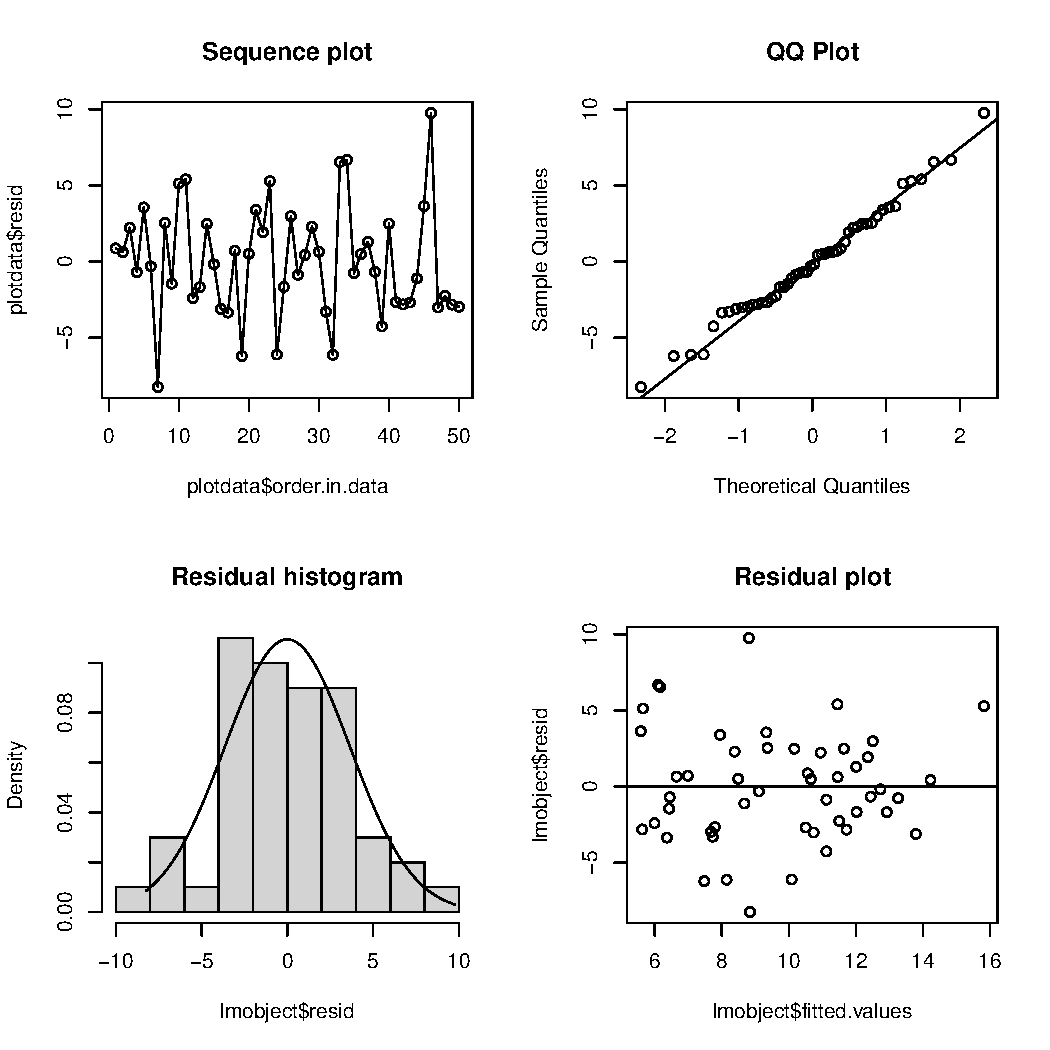
\includegraphics[width=0.6\textwidth]{figure/unnamed-chunk-1-1} 

}


\begin{kframe}\begin{alltt}
\hlcom{# Define higher-order predictors}
\hlstd{powercells} \hlkwb{<-} \hlkwd{cbind}\hlstd{(powercells,}
                    \hlkwc{cr_temp} \hlstd{= powercells}\hlopt{$}\hlstd{charge_rate} \hlopt{*} \hlstd{powercells}\hlopt{$}\hlstd{temperature,}
                    \hlkwc{cr2} \hlstd{= powercells}\hlopt{$}\hlstd{charge_rate}\hlopt{^}\hlnum{2}\hlstd{,}
                    \hlkwc{temp2} \hlstd{= powercells}\hlopt{$}\hlstd{temperature}\hlopt{^}\hlnum{2}\hlstd{)}

\hlcom{# Create a regression model with an interaction term.}
\hlcom{# NOTE: The following two lines are equivalent. The second line below is}
\hlcom{# probably "better" in the sense that it is a more efficient R way to include}
\hlcom{# an interaction term in a model.}
\hlstd{powercells_int_lm} \hlkwb{<-} \hlkwd{lm}\hlstd{(cycles} \hlopt{~} \hlstd{charge_rate} \hlopt{+} \hlstd{temperature} \hlopt{+} \hlstd{cr_temp,}
                        \hlkwc{data} \hlstd{= powercells)}
\hlstd{powercells_int_lm} \hlkwb{<-} \hlkwd{lm}\hlstd{(cycles} \hlopt{~} \hlstd{charge_rate}\hlopt{*}\hlstd{temperature,} \hlkwc{data} \hlstd{= powercells)}

\hlkwd{anova}\hlstd{(powercells_int_lm)}
\end{alltt}
\begin{verbatim}
## Analysis of Variance Table
## 
## Response: cycles
##                         Df Sum Sq Mean Sq F value    Pr(>F)    
## charge_rate              1  18704   18704 18.2573 0.0036877 ** 
## temperature              1  34201   34201 33.3844 0.0006787 ***
## charge_rate:temperature  1    529     529  0.5164 0.4956777    
## Residuals                7   7171    1024                      
## ---
## Signif. codes:  0 '***' 0.001 '**' 0.01 '*' 0.05 '.' 0.1 ' ' 1
\end{verbatim}
\begin{alltt}
\hlcom{# Create a regression model with all higher-order predictors}
\hlstd{powercells_higher_lm} \hlkwb{<-} \hlkwd{lm}\hlstd{(cycles} \hlopt{~} \hlstd{charge_rate} \hlopt{+} \hlstd{temperature} \hlopt{+} \hlstd{cr_temp} \hlopt{+}
                             \hlstd{cr2} \hlopt{+} \hlstd{temp2,} \hlkwc{data} \hlstd{= powercells)}

\hlcom{# Test the null hypothesis that cr_temp = cr2 = temp2 = 0}
\hlcom{# (This tests to see if there is any sort of higher-order interaction going}
\hlcom{# on here)}

\hlcom{# To test the above null hypothesis, we create a reduced model that is missing}
\hlcom{# the above higher order predictors, then we call the ANOVA function with}
\hlcom{# the two models to compare them.}
\hlstd{powercells_reduced_lm} \hlkwb{<-} \hlkwd{lm}\hlstd{(cycles} \hlopt{~} \hlstd{.} \hlopt{-}\hlstd{cr_temp} \hlopt{-}\hlstd{cr2} \hlopt{-}\hlstd{temp2,} \hlkwc{data} \hlstd{= powercells)}
\hlkwd{anova}\hlstd{(powercells_higher_lm, powercells_reduced_lm)}
\end{alltt}
\begin{verbatim}
## Analysis of Variance Table
## 
## Model 1: cycles ~ charge_rate + temperature + cr_temp + cr2 + temp2
## Model 2: cycles ~ (charge_rate + temperature + cr_temp + cr2 + temp2) - 
##     cr_temp - cr2 - temp2
##   Res.Df    RSS Df Sum of Sq      F Pr(>F)
## 1      5 5240.4                           
## 2      8 7700.3 -3   -2459.9 0.7823 0.5527
\end{verbatim}
\begin{alltt}
\hlcom{# Above we get a p-value of 0.4957 which tells us that we would fail to reject}
\hlcom{# the null hypothesis that all higher-order interaction terms are 0}
\end{alltt}
\end{kframe}
\end{knitrout}

\subsubsection*{Look at higher-order variables, but standardize first}

\begin{knitrout}
\definecolor{shadecolor}{rgb}{0.969, 0.969, 0.969}\color{fgcolor}\begin{kframe}
\begin{alltt}
\hlcom{# Standardize first}
\hlstd{powercells_stdz} \hlkwb{<-} \hlkwd{data.frame}\hlstd{(}\hlkwd{scale}\hlstd{(powercells))}
\hlstd{powercells_stdz}\hlopt{$}\hlstd{cr_temp} \hlkwb{<-} \hlstd{powercells_stdz}\hlopt{$}\hlstd{charge_rate} \hlopt{*} \hlstd{powercells_stdz}\hlopt{$}\hlstd{temperature}
\hlstd{powercells_stdz}\hlopt{$}\hlstd{cr2} \hlkwb{<-} \hlstd{powercells_stdz}\hlopt{$}\hlstd{charge_rate}\hlopt{^}\hlnum{2}
\hlstd{powercells_stdz}\hlopt{$}\hlstd{temp2} \hlkwb{<-} \hlstd{powercells_stdz}\hlopt{$}\hlstd{temperature}\hlopt{^}\hlnum{2}

\hlcom{# look for an interaction by looking at the ANOVA table}
\hlstd{powercells_stdz_lm} \hlkwb{<-} \hlkwd{lm}\hlstd{(cycles} \hlopt{~} \hlstd{charge_rate} \hlopt{+} \hlstd{temperature} \hlopt{+} \hlstd{cr_temp,}
                         \hlkwc{data} \hlstd{= powercells_stdz)}
\hlkwd{anova}\hlstd{(powercells_stdz_lm)}
\end{alltt}
\begin{verbatim}
## Analysis of Variance Table
## 
## Response: cycles
##             Df Sum Sq Mean Sq F value    Pr(>F)    
## charge_rate  1 3.0862  3.0862 18.2573 0.0036877 ** 
## temperature  1 5.6433  5.6433 33.3844 0.0006787 ***
## cr_temp      1 0.0873  0.0873  0.5164 0.4956777    
## Residuals    7 1.1833  0.1690                      
## ---
## Signif. codes:  0 '***' 0.001 '**' 0.01 '*' 0.05 '.' 0.1 ' ' 1
\end{verbatim}
\begin{alltt}
\hlcom{# (Our p-value checking for the interaction term above would be 0.4957)}

\hlcom{# Check for the presence of higher-order predictor significance. Again,}
\hlcom{# we accomplish this by creating a model that includes all terms and all higher}
\hlcom{# order terms, and creating another model that does not have any higher order}
\hlcom{# terms. We can then pass in the two models into the ANOVA function to test}
\hlcom{# the null hypothesis that all the higher order coefficients are 0.}
\hlstd{powercells_stdz_all_terms} \hlkwb{<-} \hlkwd{lm}\hlstd{(cycles} \hlopt{~} \hlstd{.,} \hlkwc{data} \hlstd{= powercells_stdz)}
\hlstd{powercells_stdz_no_higher} \hlkwb{<-} \hlkwd{lm}\hlstd{(cycles} \hlopt{~} \hlstd{.} \hlopt{-}\hlstd{cr2} \hlopt{-}\hlstd{temp2} \hlopt{-}\hlstd{cr_temp,} \hlkwc{data} \hlstd{= powercells_stdz)}
\hlkwd{anova}\hlstd{(powercells_stdz_all_terms, powercells_stdz_no_higher)}
\end{alltt}
\begin{verbatim}
## Analysis of Variance Table
## 
## Model 1: cycles ~ charge_rate + temperature + cr_temp + cr2 + temp2
## Model 2: cycles ~ (charge_rate + temperature + cr_temp + cr2 + temp2) - 
##     cr2 - temp2 - cr_temp
##   Res.Df     RSS Df Sum of Sq      F Pr(>F)
## 1      5 0.86467                           
## 2      8 1.27056 -3  -0.40588 0.7823 0.5527
\end{verbatim}
\begin{alltt}
\hlcom{# Above our p-value for the test would be 0.5527}
\end{alltt}
\end{kframe}
\end{knitrout}

Ending note: You don't need to standardize predictors to look at higher-order predictors like this. Instead, you can include a higher-order predictor and test it; if not significant, drop it; if significant, don't worry about significance of lower-order term. If higher-order term is significant and you really need to look at significance of lower-order term, or if the context of the data would allow the lower-order and higher-order terms to be 'stand-alone' interpretable, then standardize.

Tests for higher-order terms are the same whether data are standardized or not.

\newpage

\textbf{Example 2:} An economist wishes to relate the speed with which a particular insurance innovation is adopted ($Y$, in months) to the size of the insurance firm ($X_1$, in millions of dollars) and the type of firm ($X_2$, either mutual (0) or stock firms (1)).

\begin{knitrout}
\definecolor{shadecolor}{rgb}{0.969, 0.969, 0.969}\color{fgcolor}\begin{kframe}
\begin{alltt}
\hlcom{# Load the data}
\hlkwd{data}\hlstd{(insurance)}
\hlkwd{head}\hlstd{(insurance)}
\end{alltt}
\begin{verbatim}
##   months size type
## 1     17  151    0
## 2     26   92    0
## 3     21  175    0
## 4     30   31    0
## 5     22  104    0
## 6      0  277    0
\end{verbatim}
\begin{alltt}
\hlcom{# Model with only the quantitative predictor}
\hlstd{insurance_lm_quant} \hlkwb{<-} \hlkwd{lm}\hlstd{(months} \hlopt{~} \hlstd{size,} \hlkwc{data} \hlstd{= insurance)}
\hlkwd{summary}\hlstd{(insurance_lm_quant)}
\end{alltt}
\begin{verbatim}
## 
## Call:
## lm(formula = months ~ size, data = insurance)
## 
## Residuals:
##      Min       1Q   Median       3Q      Max 
## -10.4621  -4.7236   0.7912   4.3427   7.9055 
## 
## Coefficients:
##             Estimate Std. Error t value Pr(>|t|)    
## (Intercept) 36.48211    2.84425  12.827 1.71e-10 ***
## size        -0.09394    0.01426  -6.589 3.45e-06 ***
## ---
## Signif. codes:  0 '***' 0.001 '**' 0.01 '*' 0.05 '.' 0.1 ' ' 1
## 
## Residual standard error: 5.231 on 18 degrees of freedom
## Multiple R-squared:  0.7069,	Adjusted R-squared:  0.6906 
## F-statistic: 43.41 on 1 and 18 DF,  p-value: 3.452e-06
\end{verbatim}
\begin{alltt}
\hlcom{# Model with only the qualitative predictor}
\hlstd{insurance_lm_qual} \hlkwb{<-} \hlkwd{lm}\hlstd{(months} \hlopt{~} \hlstd{type,} \hlkwc{data} \hlstd{= insurance)}
\hlkwd{summary}\hlstd{(insurance_lm_qual)}
\end{alltt}
\begin{verbatim}
## 
## Call:
## lm(formula = months ~ type, data = insurance)
## 
## Residuals:
##    Min     1Q Median     3Q    Max 
## -16.70  -7.35  -0.20   6.40  15.90 
## 
## Coefficients:
##             Estimate Std. Error t value Pr(>|t|)    
## (Intercept)    16.70       2.92   5.719 2.02e-05 ***
## type            5.40       4.13   1.308    0.207    
## ---
## Signif. codes:  0 '***' 0.001 '**' 0.01 '*' 0.05 '.' 0.1 ' ' 1
## 
## Residual standard error: 9.235 on 18 degrees of freedom
## Multiple R-squared:  0.08674,	Adjusted R-squared:  0.03601 
## F-statistic:  1.71 on 1 and 18 DF,  p-value: 0.2075
\end{verbatim}
\begin{alltt}
\hlcom{# Create a boxplot of the variable "months" by the two different types}
\hlkwd{boxplot}\hlstd{(months} \hlopt{~} \hlstd{type,} \hlkwc{data} \hlstd{= insurance,}
        \hlkwc{main} \hlstd{=} \hlstr{"Distribution of months by type"}\hlstd{)}
\end{alltt}
\end{kframe}

{\centering 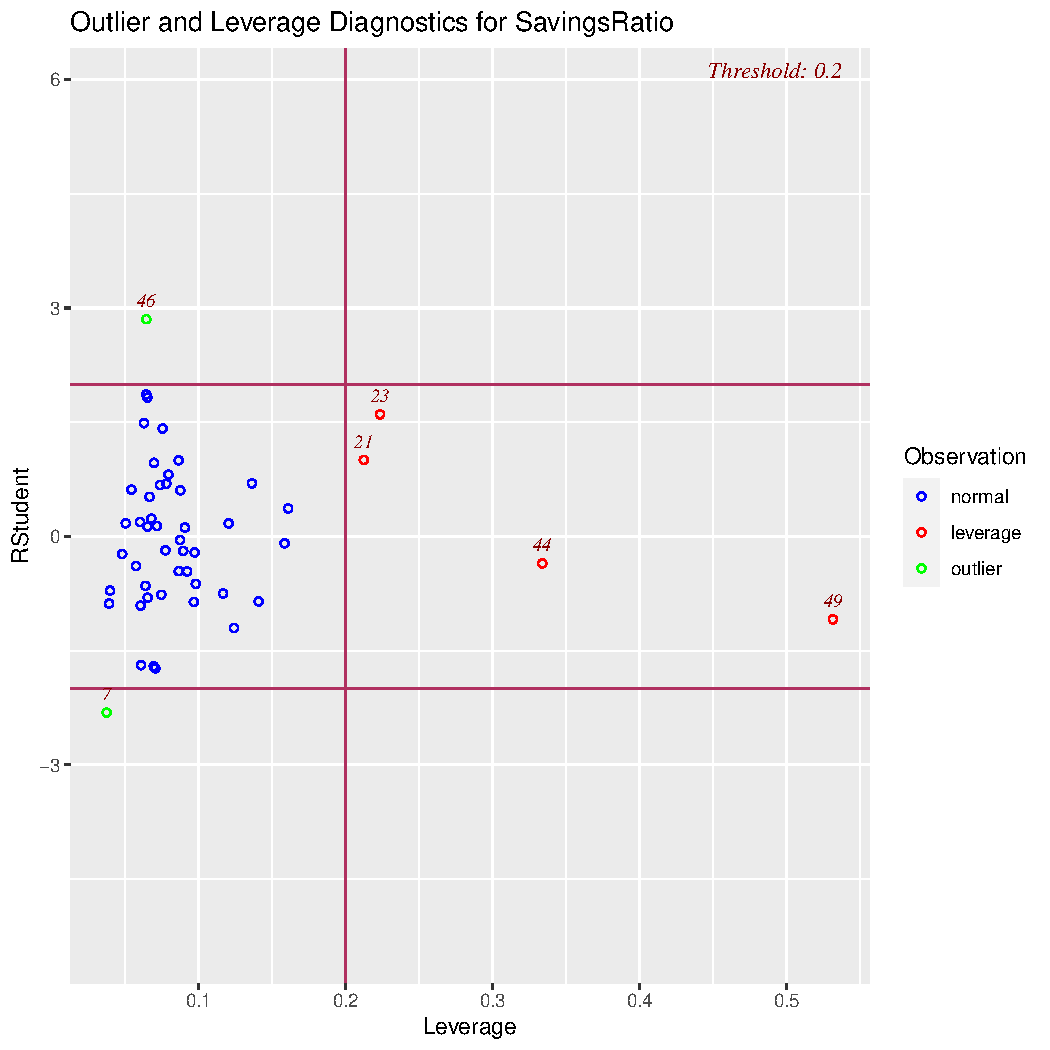
\includegraphics[width=0.6\textwidth]{figure/unnamed-chunk-3-1} 

}



\end{knitrout}

\subsubsection*{Create a linear model (no interaction present):}

\begin{knitrout}
\definecolor{shadecolor}{rgb}{0.969, 0.969, 0.969}\color{fgcolor}\begin{kframe}
\begin{alltt}
\hlcom{# Create the additive model with both predictor types}
\hlstd{insurance_lm} \hlkwb{<-} \hlkwd{lm}\hlstd{(months} \hlopt{~} \hlstd{size} \hlopt{+} \hlstd{type,} \hlkwc{data} \hlstd{= insurance)}
\hlkwd{summary}\hlstd{(insurance_lm)}
\end{alltt}
\begin{verbatim}
## 
## Call:
## lm(formula = months ~ size + type, data = insurance)
## 
## Residuals:
##     Min      1Q  Median      3Q     Max 
## -5.6915 -1.7036 -0.4385  1.9210  6.3406 
## 
## Coefficients:
##              Estimate Std. Error t value Pr(>|t|)    
## (Intercept) 33.874069   1.813858  18.675 9.15e-13 ***
## size        -0.101742   0.008891 -11.443 2.07e-09 ***
## type         8.055469   1.459106   5.521 3.74e-05 ***
## ---
## Signif. codes:  0 '***' 0.001 '**' 0.01 '*' 0.05 '.' 0.1 ' ' 1
## 
## Residual standard error: 3.221 on 17 degrees of freedom
## Multiple R-squared:  0.8951,	Adjusted R-squared:  0.8827 
## F-statistic:  72.5 on 2 and 17 DF,  p-value: 4.765e-09
\end{verbatim}
\begin{alltt}
\hlcom{# Create a fit plot individually for each of the two type levels. This isn't}
\hlcom{# something that's natively supported in R or the stat5100 package, so we}
\hlcom{# will have to grab the coefficients manually from the linear model.}

\hlcom{# Each of these vectors below contain (intercept, slope). Note that in the}
\hlcom{# type1, we find the intercept by adding the estimate of "type" onto the}
\hlcom{# existing intercept}
\hlstd{type0_coeff} \hlkwb{<-} \hlkwd{c}\hlstd{(}\hlnum{33.874069}\hlstd{,} \hlopt{-}\hlnum{0.101742}\hlstd{)}
\hlstd{type1_coeff} \hlkwb{<-} \hlkwd{c}\hlstd{(}\hlnum{33.874069} \hlopt{+} \hlnum{8.055469}\hlstd{,} \hlopt{-}\hlnum{0.101742}\hlstd{)}

\hlcom{# Type 0}
\hlstd{type0} \hlkwb{<-} \hlstd{insurance[insurance}\hlopt{$}\hlstd{type} \hlopt{==} \hlnum{0}\hlstd{, ]}
\hlkwd{plot}\hlstd{(type0}\hlopt{$}\hlstd{size, type0}\hlopt{$}\hlstd{months,} \hlkwc{col} \hlstd{=} \hlstr{"red"}\hlstd{,} \hlkwc{main} \hlstd{=} \hlstr{"Additive model"}\hlstd{,}
     \hlkwc{xlab} \hlstd{=} \hlstr{"Size"}\hlstd{,} \hlkwc{ylab} \hlstd{=} \hlstr{"Months"}\hlstd{)}
\hlkwd{abline}\hlstd{(}\hlkwc{a} \hlstd{= type0_coeff[}\hlnum{1}\hlstd{],} \hlkwc{b} \hlstd{= type0_coeff[}\hlnum{2}\hlstd{],} \hlkwc{col} \hlstd{=} \hlstr{"red"}\hlstd{)}

\hlcom{# Type 1}
\hlstd{type1} \hlkwb{<-} \hlstd{insurance[insurance}\hlopt{$}\hlstd{type} \hlopt{==} \hlnum{1}\hlstd{, ]}
\hlkwd{points}\hlstd{(type1}\hlopt{$}\hlstd{size, type1}\hlopt{$}\hlstd{months,} \hlkwc{col} \hlstd{=} \hlstr{"blue"}\hlstd{)}
\hlkwd{abline}\hlstd{(}\hlkwc{a} \hlstd{= type1_coeff[}\hlnum{1}\hlstd{],} \hlkwc{b} \hlstd{= type1_coeff[}\hlnum{2}\hlstd{],} \hlkwc{col} \hlstd{=} \hlstr{"blue"}\hlstd{)}

\hlcom{# Add a legend}
\hlkwd{legend}\hlstd{(}\hlkwc{x} \hlstd{=} \hlnum{50}\hlstd{,} \hlkwc{y} \hlstd{=} \hlnum{7}\hlstd{,} \hlkwd{c}\hlstd{(}\hlstr{"Type 0"}\hlstd{,}\hlstr{"Type 1"}\hlstd{),} \hlkwc{cex} \hlstd{=} \hlnum{1.2}\hlstd{,}
       \hlkwc{col} \hlstd{=} \hlkwd{c}\hlstd{(}\hlstr{"red"}\hlstd{,} \hlstr{"blue"}\hlstd{),} \hlkwc{pch} \hlstd{=} \hlkwd{c}\hlstd{(}\hlnum{1}\hlstd{,}\hlnum{1}\hlstd{))}
\end{alltt}
\end{kframe}

{\centering 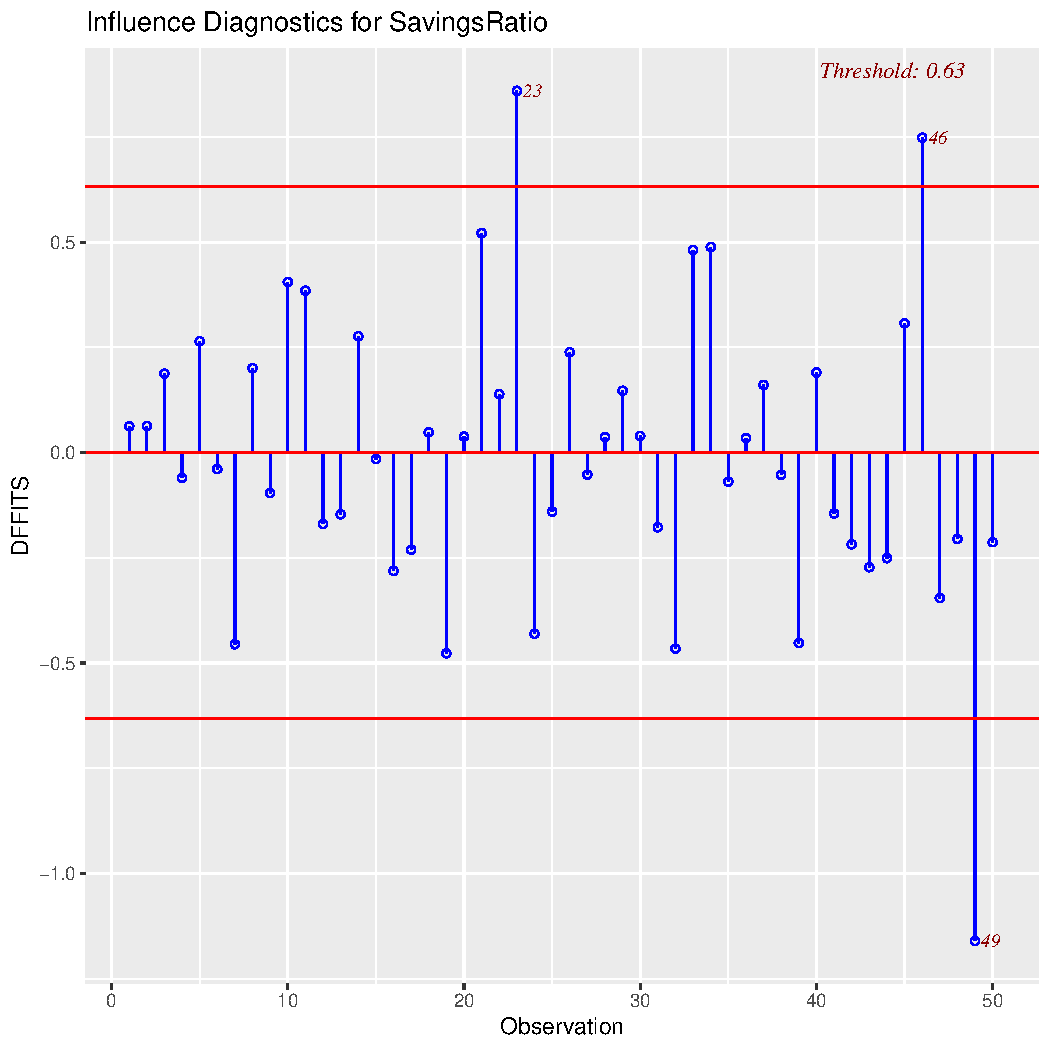
\includegraphics[width=0.6\textwidth]{figure/unnamed-chunk-4-1} 

}



\end{knitrout}

\newpage
\subsubsection*{Create an interaction model:}

\begin{knitrout}
\definecolor{shadecolor}{rgb}{0.969, 0.969, 0.969}\color{fgcolor}\begin{kframe}
\begin{alltt}
\hlcom{# Create an interaction model}
\hlstd{insurance_int_lm} \hlkwb{<-} \hlkwd{lm}\hlstd{(months} \hlopt{~} \hlstd{size}\hlopt{*}\hlstd{type,} \hlkwc{data} \hlstd{= insurance)}
\hlkwd{summary}\hlstd{(insurance_int_lm)}
\end{alltt}
\begin{verbatim}
## 
## Call:
## lm(formula = months ~ size * type, data = insurance)
## 
## Residuals:
##     Min      1Q  Median      3Q     Max 
## -5.7144 -1.7064 -0.4557  1.9311  6.3259 
## 
## Coefficients:
##               Estimate Std. Error t value Pr(>|t|)    
## (Intercept) 33.8383695  2.4406498  13.864 2.47e-10 ***
## size        -0.1015306  0.0130525  -7.779 7.97e-07 ***
## type         8.1312501  3.6540517   2.225   0.0408 *  
## size:type   -0.0004171  0.0183312  -0.023   0.9821    
## ---
## Signif. codes:  0 '***' 0.001 '**' 0.01 '*' 0.05 '.' 0.1 ' ' 1
## 
## Residual standard error: 3.32 on 16 degrees of freedom
## Multiple R-squared:  0.8951,	Adjusted R-squared:  0.8754 
## F-statistic: 45.49 on 3 and 16 DF,  p-value: 4.675e-08
\end{verbatim}
\begin{alltt}
\hlcom{# To include the interaction in a similar plot above, we change the}
\hlcom{# slope of the type 1 line to be the sum of the estimate for type and the}
\hlcom{# estimate for the interaction coefficient.}
\hlstd{type0_coeff} \hlkwb{<-} \hlkwd{c}\hlstd{(}\hlnum{33.8383695}\hlstd{,} \hlopt{-}\hlnum{0.1015306}\hlstd{)}
\hlstd{type1_coeff} \hlkwb{<-} \hlkwd{c}\hlstd{(}\hlnum{33.8383695} \hlopt{+} \hlnum{8.1312501}\hlstd{,} \hlopt{-}\hlnum{0.1015306} \hlopt{-} \hlnum{0.0004171}\hlstd{)}

\hlcom{# Type 0}
\hlstd{type0} \hlkwb{<-} \hlstd{insurance[insurance}\hlopt{$}\hlstd{type} \hlopt{==} \hlnum{0}\hlstd{, ]}
\hlkwd{plot}\hlstd{(type0}\hlopt{$}\hlstd{size, type0}\hlopt{$}\hlstd{months,} \hlkwc{col} \hlstd{=} \hlstr{"red"}\hlstd{,} \hlkwc{main} \hlstd{=} \hlstr{"Additive model"}\hlstd{,}
     \hlkwc{xlab} \hlstd{=} \hlstr{"Size"}\hlstd{,} \hlkwc{ylab} \hlstd{=} \hlstr{"Months"}\hlstd{)}
\hlkwd{abline}\hlstd{(}\hlkwc{a} \hlstd{= type0_coeff[}\hlnum{1}\hlstd{],} \hlkwc{b} \hlstd{= type0_coeff[}\hlnum{2}\hlstd{],} \hlkwc{col} \hlstd{=} \hlstr{"red"}\hlstd{)}

\hlcom{# Type 1}
\hlstd{type1} \hlkwb{<-} \hlstd{insurance[insurance}\hlopt{$}\hlstd{type} \hlopt{==} \hlnum{1}\hlstd{, ]}
\hlkwd{points}\hlstd{(type1}\hlopt{$}\hlstd{size, type1}\hlopt{$}\hlstd{months,} \hlkwc{col} \hlstd{=} \hlstr{"blue"}\hlstd{)}
\hlkwd{abline}\hlstd{(}\hlkwc{a} \hlstd{= type1_coeff[}\hlnum{1}\hlstd{],} \hlkwc{b} \hlstd{= type1_coeff[}\hlnum{2}\hlstd{],} \hlkwc{col} \hlstd{=} \hlstr{"blue"}\hlstd{)}

\hlcom{# Add a legend}
\hlkwd{legend}\hlstd{(}\hlkwc{x} \hlstd{=} \hlnum{50}\hlstd{,} \hlkwc{y} \hlstd{=} \hlnum{7}\hlstd{,} \hlkwd{c}\hlstd{(}\hlstr{"Type 0"}\hlstd{,}\hlstr{"Type 1"}\hlstd{),} \hlkwc{cex} \hlstd{=} \hlnum{1.2}\hlstd{,}
       \hlkwc{col} \hlstd{=} \hlkwd{c}\hlstd{(}\hlstr{"red"}\hlstd{,} \hlstr{"blue"}\hlstd{),} \hlkwc{pch} \hlstd{=} \hlkwd{c}\hlstd{(}\hlnum{1}\hlstd{,}\hlnum{1}\hlstd{))}
\end{alltt}
\end{kframe}

{\centering 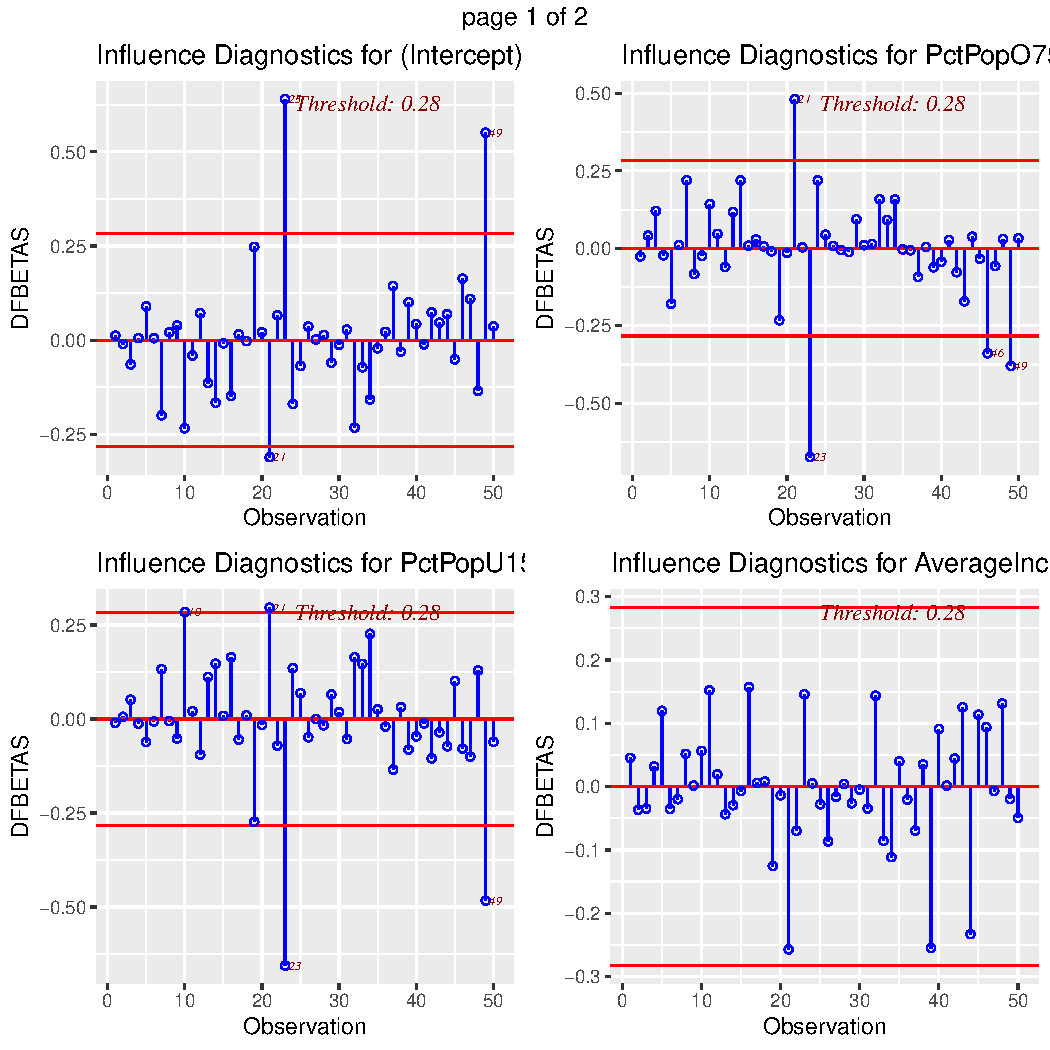
\includegraphics[width=0.6\textwidth]{figure/unnamed-chunk-5-1} 

}



\end{knitrout}

\end{document}
